\documentclass{article} % For LaTeX2e
% \usepackage{nips13submit_e,times}
\usepackage{hyperref}
\usepackage{url}
\usepackage{graphicx}
\usepackage{amsmath}
\usepackage{float}
%\documentstyle[nips13submit_09,times,art10]{article} % For LaTeX 2.09


\title{Traffic Flow Maximization using Evolutionary Algorithm}


\newcommand{\fix}{\marginpar{FIX}}
\newcommand{\new}{\marginpar{NEW}}

\begin{document}


\maketitle

\begin{abstract}
Traffic Flow maximization is one of the crucial problems in designing a city. It directly affects the daily life of the people living in that city. It is a complex problem, one that in most cases cannot be deterministically solved. We propose using evolutionary algorithms to solve that problem. We compare existing work and traffic flow with solutions yielded by our evolutionary approach, and our results show that it is beneficial to adopt this strategy when designing traffic light timings.
\end{abstract}

\section{Scope of the Problem}

Traffic infrastructure comes in various forms, and optimizing traffic flow in road networks is a task that depends highly on the infrastructure. We commonly consider infrastructure as being in one of two categories:  ``smart'' infrastructure and ``legacy'' infrastructure. The first makes use of detectors placed in the infrastructure to determine the state of traffic, whereas the second does not.

It is reasonable to assume that achieved solutions will perform better as a whole when making use of smart infrastructure. For example, a traffic light that can detect that there is no traffic from East to West, and that vehicles are waiting to go from North to South, can react accordingly and change its state to shorten the wait of these vehicles.

There have been projects in the past where traffic flow was optimized by combining real-time knowledge of traffic and communication between lights. The best-known of these projects is one spearheaded by Carnegie Mellon University in the East Liberty part of Pittsburgh, with excellent results.

However, this previous study's approach relies heavily on smart traffic lights and detectors, which, although quite practical, are still far and few between throughout the world. In countries such as China or India, where the number of vehicles is growing most rapidly, most roads are equipped with legacy traffic equipment.

An effective approach to solving this problem should be applicable to the maximum amount of scenarios, which is why this paper discusses only optimizing traffic light timings in a legacy environment.
However, operating in a legacy environment does not mean that we must forgo all knowledge of the traffic flow. It is reasonable to assume that traffic flow can be measured at specific intersections. The collection of this data can unearth trends in the traffic flow (ie: rush hour traffic). Once this data is collected, any period of time can be split into different sections, where each of these sections has a different, but constant, traffic flow.


In our analysis, we place ourselves in an environment where the traffic flow is a fixed parameter. The above analysis shows that this scenario is relevant.

\section{Existing Domain Research}
Research on traffic lights optimization began since the emergence of traffic lights. Researchers have come up with several different ways to optimize the traffic lights such as 

\section{Simulators}
\label{gen_inst}
A common and key ingredient in developing evolutionary algorithms is the choice of a simulator. We investigated several traffic simulators (see below) and chose the one that suits our project the best.

\subsection{Simple Java Simulator}
% \begin{figure}
%  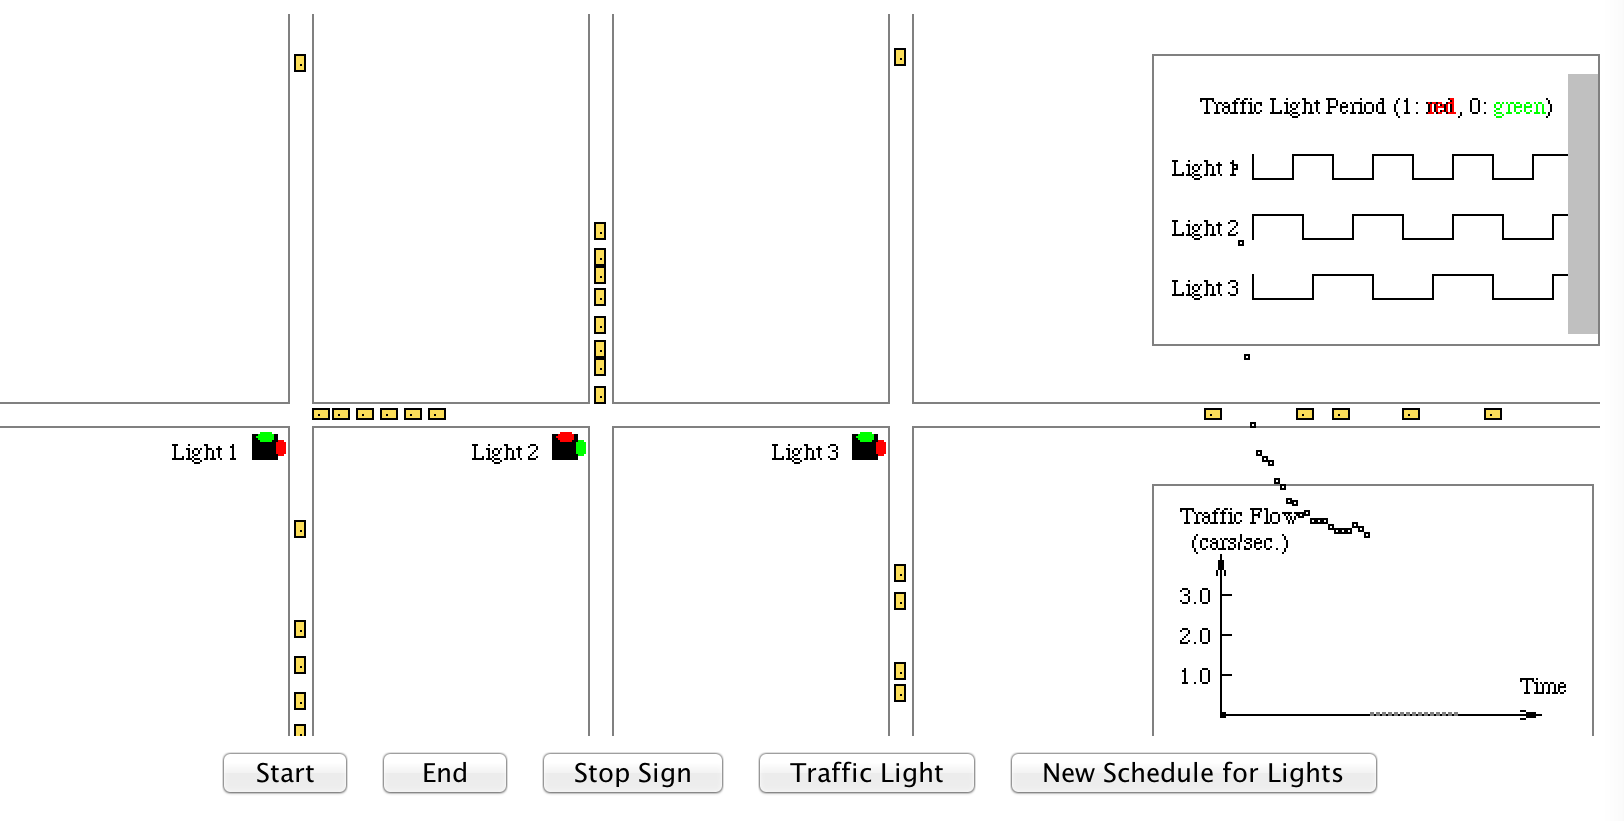
\includegraphics[width=4in]{images/simulator/SimpleJavaSimulator.png}
%  \caption{Screenshot of the Simple Java Simulator} 
% \end{figure}

This simulator can automatically generate and plot. Another feature is the ability to to drag any car from one position to another. The simulator will automatically adjust the position of the car and continue. Furthermore, it is possible to adjust in real-time the timings of traffic lights. For simple road networks and light traffic flow, it is a great choice. However, in this kind of traffic network, there isn't much to optimize, which is why we didn't choose it as our final simulator. 

\subsection{MatSim}
% \begin{figure}[]
%  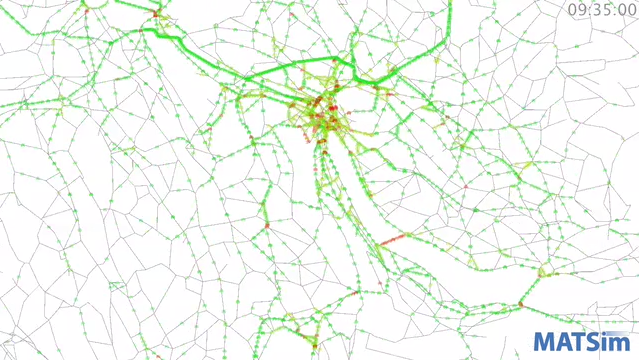
\includegraphics[width=4in]{images/simulator/matsim_zurich.png}
%  \caption{Screenshot of the Matsim simulator}
% \end{figure}

Matsim is a powerful simulator which you can see from its simulated traffic networks. 
It is open source, which means that developers can modify it as they wish and adapt it closely to their needs. Also it provides and interactive visualizer which enables users to modify the traffic networks conveniently. At the same time, it provides detailed analysis which can be used by our project.

\subsection{SUMO}
After comparing carefully among several different simulators, we finally chose SUMO which was developed by employees of the Institute of Transportation Systems at the German Aerospace Center.

\section{Simulated Traffic networks}
In order to test our algorithm, we modeled the traffic network around the Caltrain station located in Mountain View, California. This choice was informed by the fact that it is a well-known intersection among our peers and we have heard complaints about its long wait times. We investigated the traffic situation around the Caltrain station: during rush hour, we recorded the traffic flow as well as the traffic light timings.
\begin{figure}
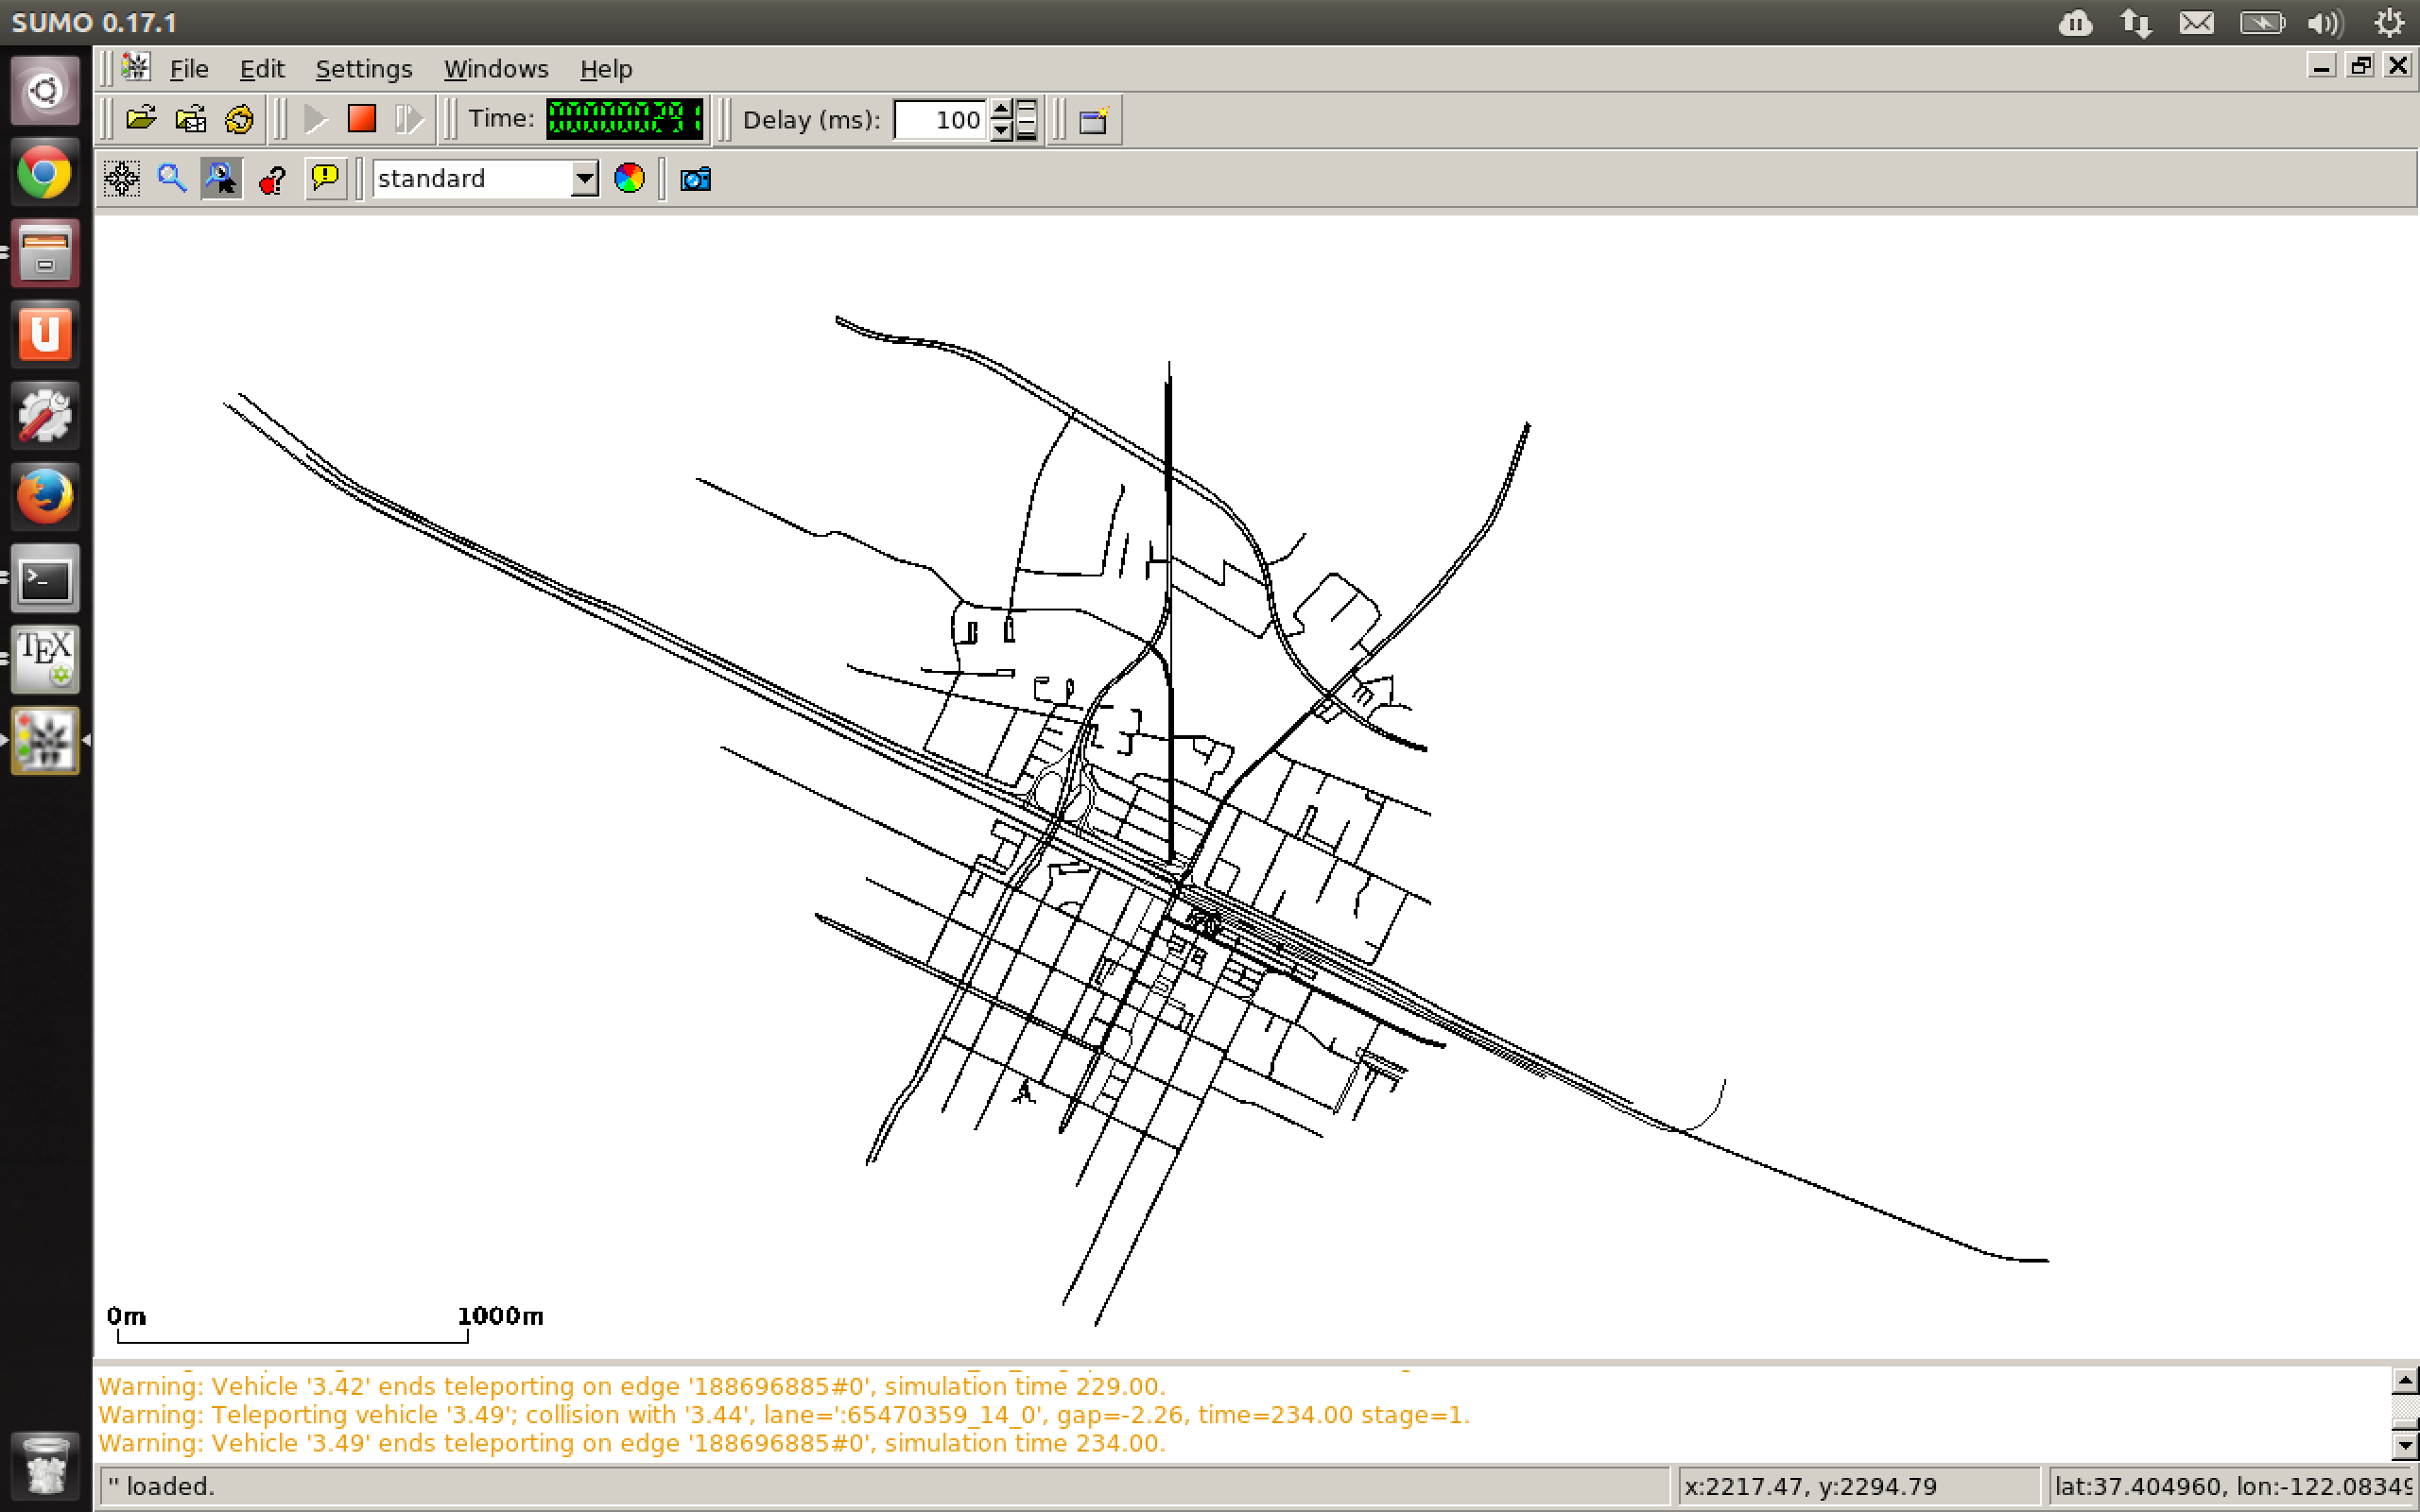
\includegraphics[width=4in]{images/simulator/caltrain.png}
\caption{Caltrain Station Simulation}
\end{figure}


\section{The choice of fitness function}
In order to best simulate the real world traffic light, we tried several ways to establish the mapping between real world traffic measurement with the fitness function in our evolutionary algorithm. The following are the fitness function we tried in our algorithm.
\subsection{Average Speed}
This is the first fitness function we tried. And it is the most intuitive one. An intuitive explanation is that if the average speed of a traffic network is larger that another, then it is more likely to have a greater traffic flow. We tried this fitness in the grid traffic network as shown in figure~\ref{fig:gridoptimum}.

\begin{figure}
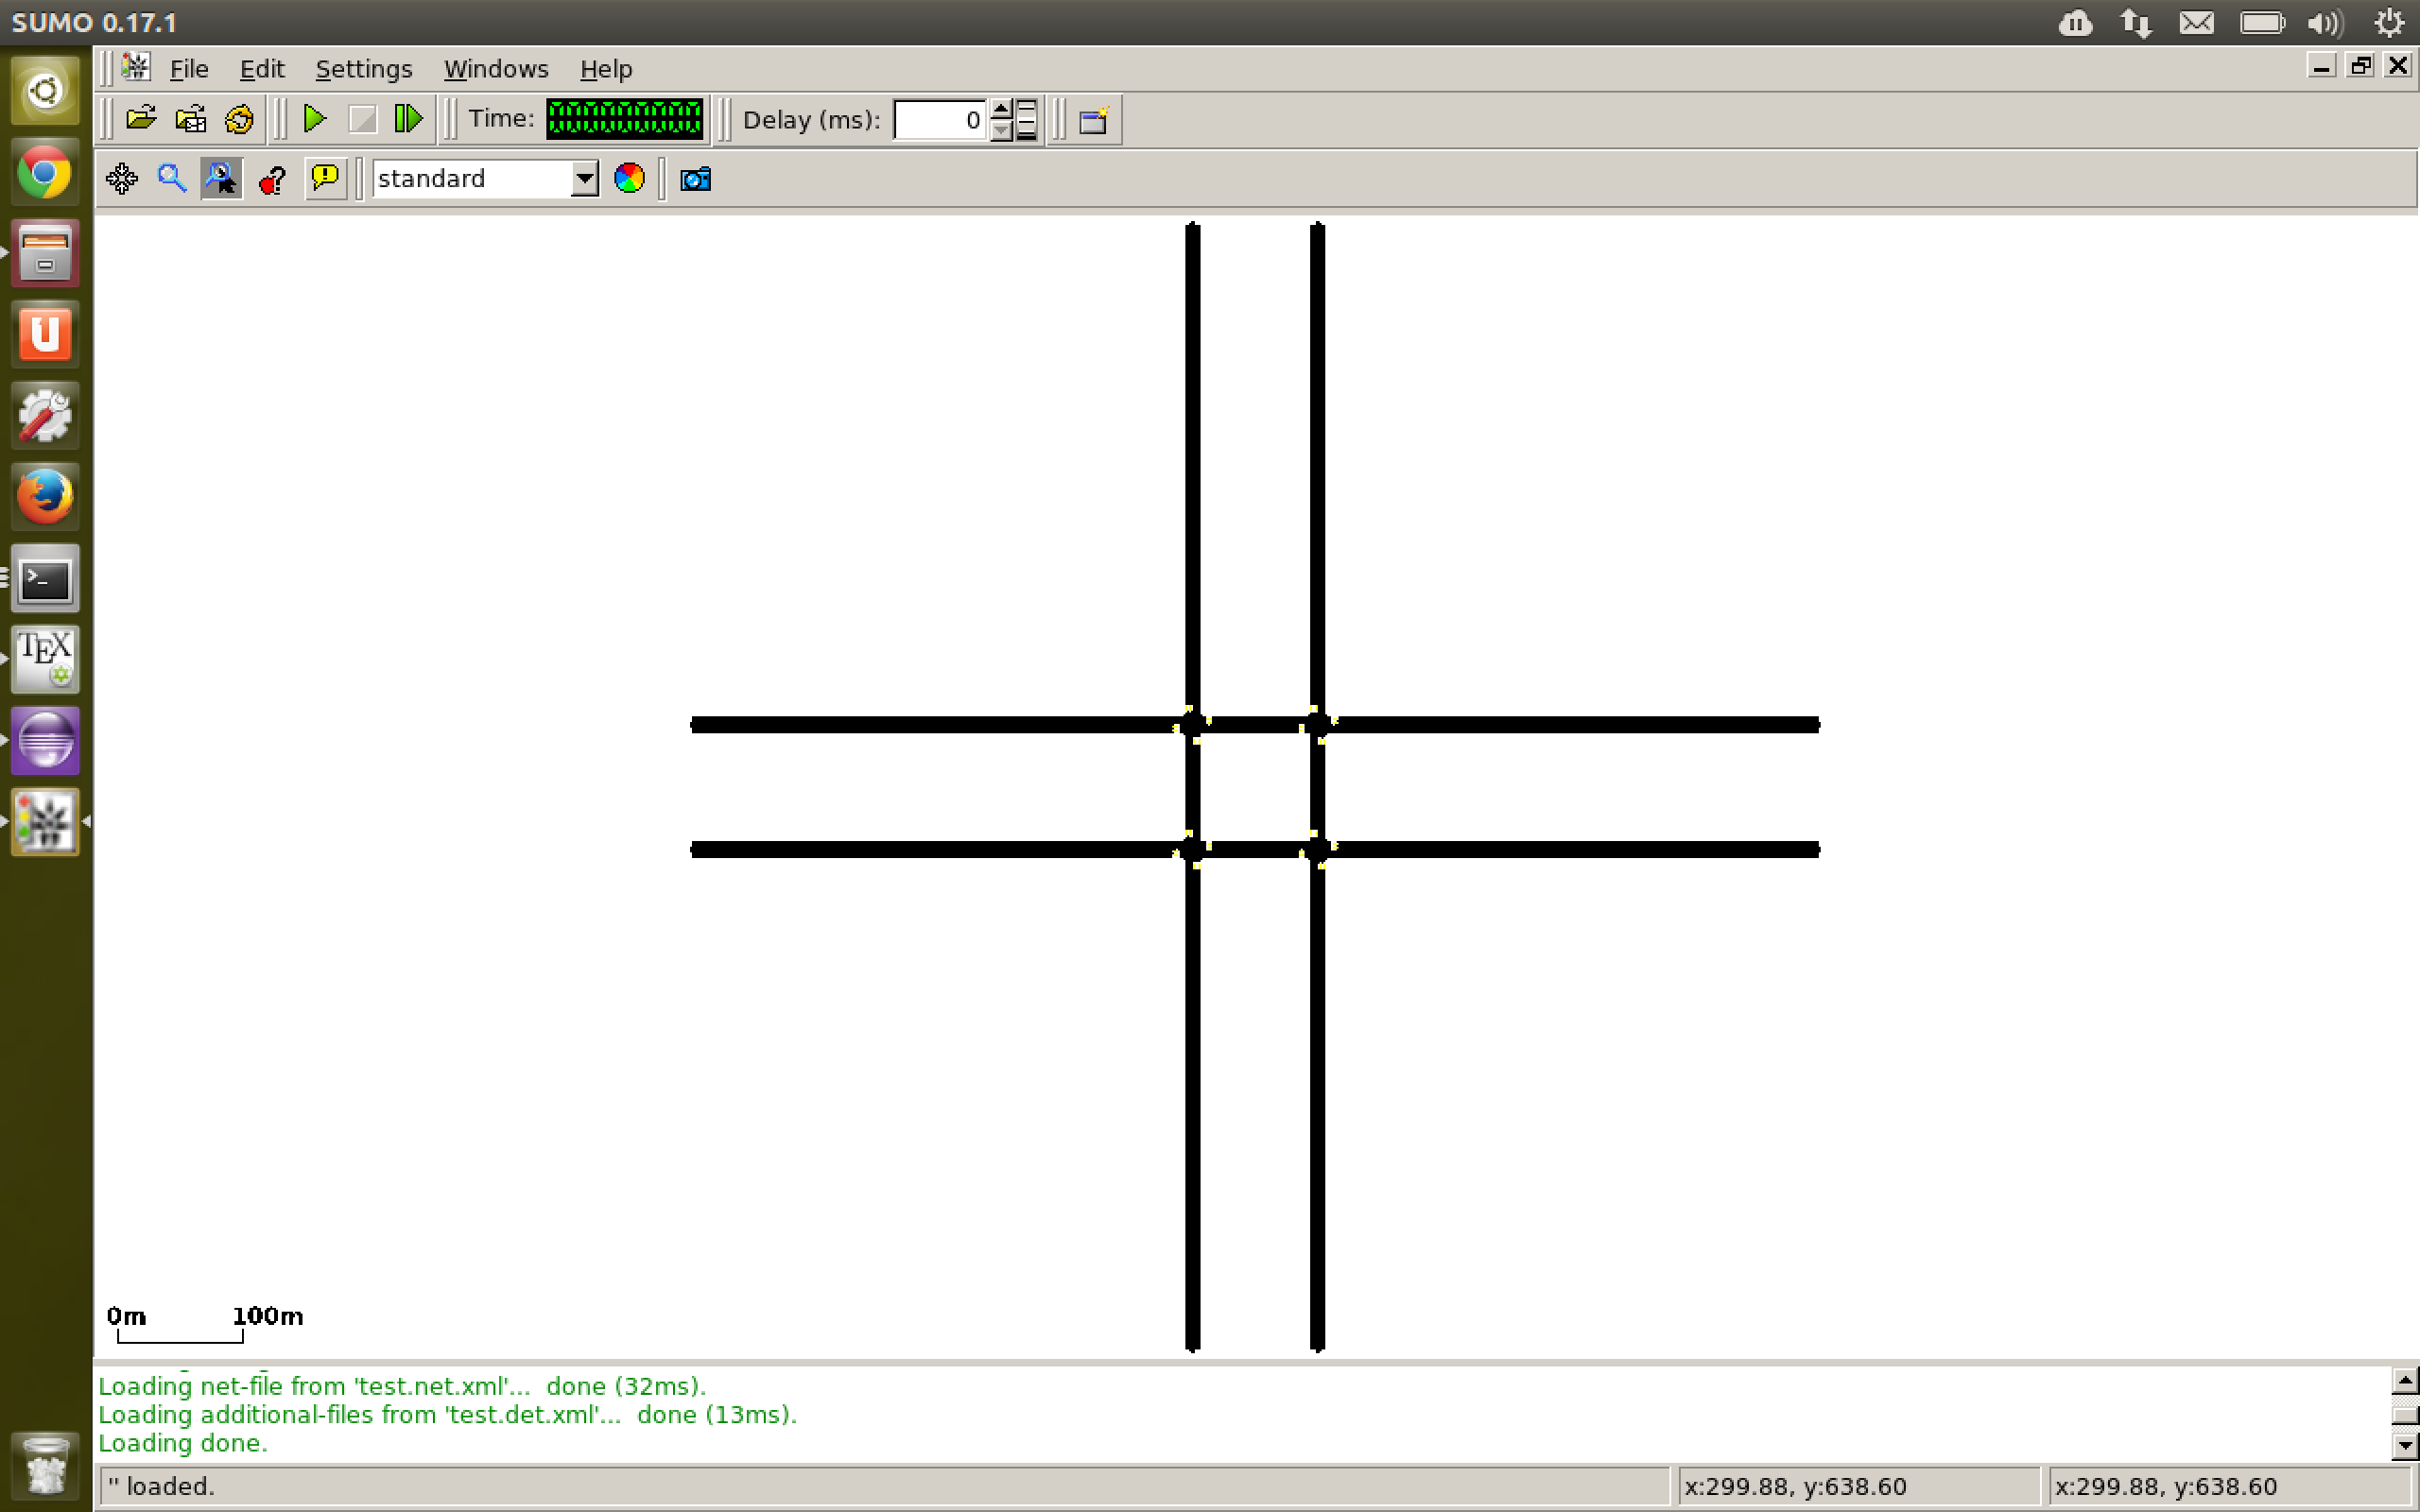
\includegraphics[width=4in]{images/simulator/gridoptimum.png}
\caption{Basic Simulation}
\label{fig:gridoptimum}
\end{figure}

\section{Algorithms}
\subsection{Genotype and Phenotype}


\subsection{Simple GA}
The first algorithm which we implemented was the Simple Genetic Algorithm. This textbook algorithm is made of several components, among which the following:
\begin{itemize}
 \item Parent Selection
 \item Recombination
 \item Mutation
 \item Survivor Selection
\end{itemize}
Each of these components can be implemented in different ways and will give the algorithm a unique behavior. Furthermore, these components make use of constants that can be tweaked (mutation rate, parent population size), just as the algorithm's parameters (population size, number of rounds). Tuning these values will also change the behavior of the alorithm.

Our implementation contains the following components:
\begin{itemize}
 \item Parent Selection: Rank-based selection, Stochastic Universal Sampling
 \item Recombination: Single Point Crossover
 \item Mutation: Simple Mutation
 \item Survivor Selector: Rank-based selection, Stochastic Universal Sampling
\end{itemize}



\subsection{Simulated Annealing}
In order to find the global optimum, we tried another algorithm which is called Simulated Annealing. The basic idea of this algorithm is to simulate the process of annealing. At the beginning, we have a high temperature in which the acceptance probability of individuals with bad fitness is high. Then temperature goes down slowly. The acceptance probability goes down as well. The way we encode our algorithm is as follows:
\begin{equation}
Simulated Annealing Gene:(T_1, T_2, T_3, T_4).
\end{equation}
Here $T_1, T_2, T_3, T_4$ represents the four traffic lights we measured around Caltrain Station respectively.
The neighbor function is defined as following:
\begin{equation}
Write the presudo code here.
\end{equation}
The function for calculating acceptance rate is:


Below is the result of using different scale factor 

\subsection{Mutable Time-interval Genetic Algorithm (MTGA)}
Our initial assumption was to work on time intervals during which the traffic flow is constant. However, after many simulations, we realized that even in a situation where the overall traffic flow is constant, the interaction between intersections and traffic lights creates a somewhat chaotic system where traffic flow at specific intersection can vary quite a bit. 

It became clear that we could achieve better results by further dividing our time intervals into smaller sub-intervals. We designed a new algorithm, in which the individuals also contain information about how to split the time interval: the Mutable Time-interval Genetic Algorithm (MTGA). It is a sort of Genetic Algorithm, and has the following features which will be explained later.
\begin{itemize}
	\item Hybrid Gene Type.
	\item No Crossover
	\item Special Mutation Type
\end{itemize}
The first and most important feature of MTGA is that it has a hybrid gene type. Below is how we encode the chromosome.
\begin{align}
Mutable Time-inverval Gene:
(&T_{1,1}, T_{1,2}, T_{1,3}, T_{1,4},\\
&T_{2,1}, T_{2,2}, T_{2,3}, T_{2,4},\\
&...,\\
&T_{n,1}, T_{n, 2}, T_{n,3}, T_{n, 4},\\
&I_1, I_2, ..., I_n).
\end{align}
In the above equation, the a in the subscript of $T_{a,b}$ represents the time for the ath time interval and b represents the bth phase of a traffic light. For simplicity, in our example, we have only 1 traffic light. This traffic light has 4 phases which is the reason that b can be 4 at max. And we subdivide the whole time interval that we want to optimize our algorithm in into  sub regions. $I_1, I_2, ...$ represents the length of each phase respectively. One thing that we have to mention is that the sum of $I_2, I_2, ...$ should be a fixed constant which represents the length of the time interval we want to estimate our algorithm in. It can be expressed like this:
\begin{equation}
\label{equ_sum_fixed}
I_2 + I_2 + I_3 + ... + I_n = T
\end{equation} 
where T represents the time interval between start time and end time.\\

Another important feature is that you cannot really perform crossover in MTGA although they align with each other very well. The reason comes from its special chromosome. Because we usually want to optimize the traffic light for a fixed time interval, therefore, $I_1 + I_2 + ... + I_n$ has to be fixed to the length of the time interval. If we perform crossover between two individuals, the sum of these numbers will change. Although we can find a way to perform crossover between two individuals, we didn't add this feature into our algorithm.

The last feature is that we have to perform special mutation in MTGA. In the first part of the chromosome, we can perform mutation as usual. However as stated above, we have to change at least two genes at together because of equation \ref{equ_sum_fixed}. For example, we want to change ${I_1}$. Let's assume that, previously, we have $I_1 = 40, I_2 = 40, I_3 = 100$. If we try to mutate$I_1$ from 40 to 20. We can set $I_1 = 20$. However, we have to do either $I_2=60$ or $I_3=120$ as well in order to keep consistent to equation:\ref{equ_sum_fixed}. 


\subsection{Fixed Time-interval Genetic Algorithm (FTGA)}
Based on the above algorithm, we came up with a modified version of the MTGA: the Fixed Time-interval Genetic Algorithm (FTGA). The simple idea is to get rid of $I_1, I_2, ..., I_n$ which are encoded in equation\ref{equ_sum_fixed}. We will ourselves decide to split the time interval into a number of equal-length sub-intervals: $I_1=I_2=...=I_n$. This means that we don't need to store the intervals in the chromosomes anymore. The chromosome's representation is the following:
\begin{align}
Fixed Time-inverval Gene:
(&T_{1,1}, T_{1,2}, T_{1,3}, T_{1,4},\\
&T_{2,1}, T_{2,2}, T_{2,3}, T_{2,4},\\
&...,\\
&T_{n,1}, T_{n, 2}, T_{n,3}, T_{n, 4})\\
\end{align}
By limiting $T_{a,b}$ to a certain domain such as (1,100), we don't even have to perform the special mutation either. What we can do with normal Genetic Algorithm can be applied to this chromosome as well. And another important feature that FTGA has is that it has fewer parameters which means it takes us a shorter time to get the result. 


\section{Experiment}
In order to test FTGA, we designed the following experiment:
\begin{itemize}
	\item Run the algorithm with different generation and compare the result with SGA and SA.
	\item change the random number generator and do the experiments for several times and compared the result with SGA and SA.
	In all the experiments, the traffic flow is the same. And the simulation step is 600. The fitness evaluation function we used is the throughput of the system.
	
\end{itemize}


\section{Results}
Below are two sets of experiments we did.
\begin{figure}[H]
\centering
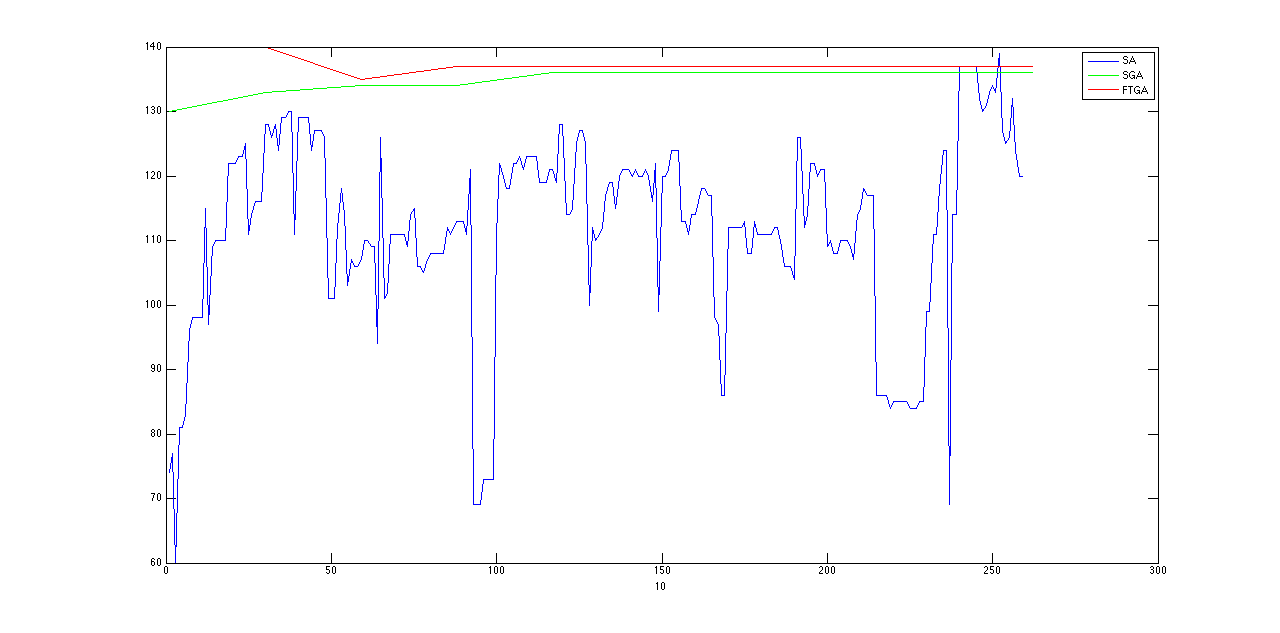
\includegraphics[scale=0.3]{images/FTGA/exp1/10.png}
\caption{Generation = 10}
\end{figure}
\begin{figure}[H]
\centering
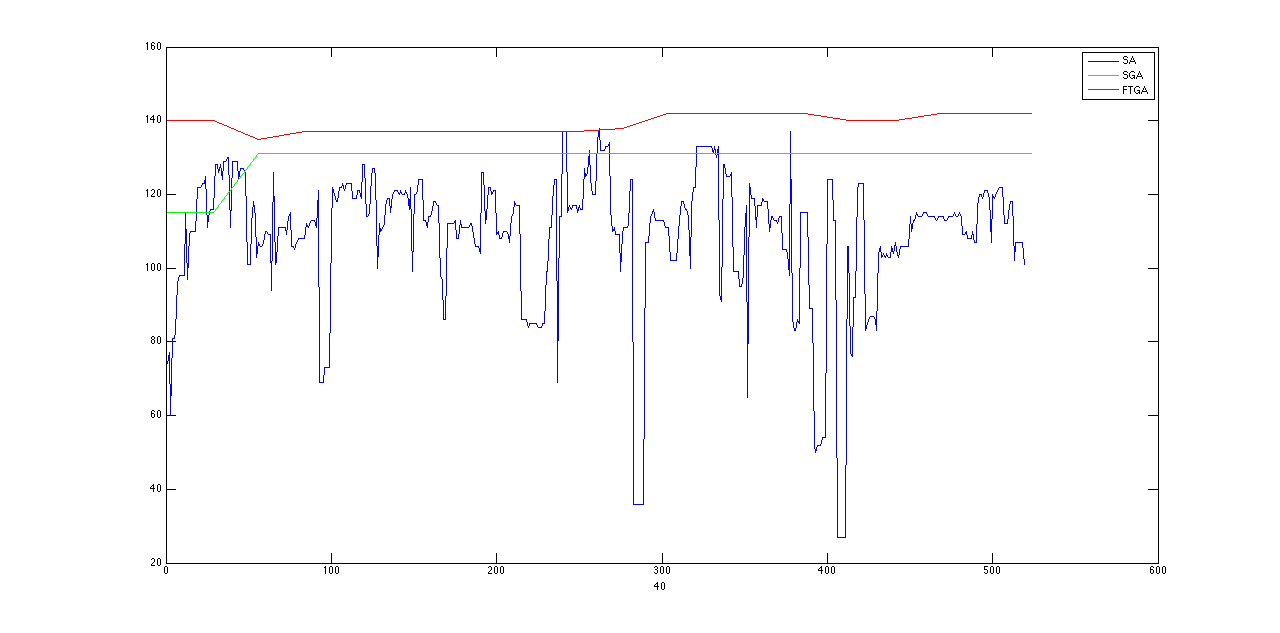
\includegraphics[scale=0.3]{images/FTGA/exp1/20.png}
\caption{Generation = 20}
\end{figure}
\begin{figure}[H]
\centering
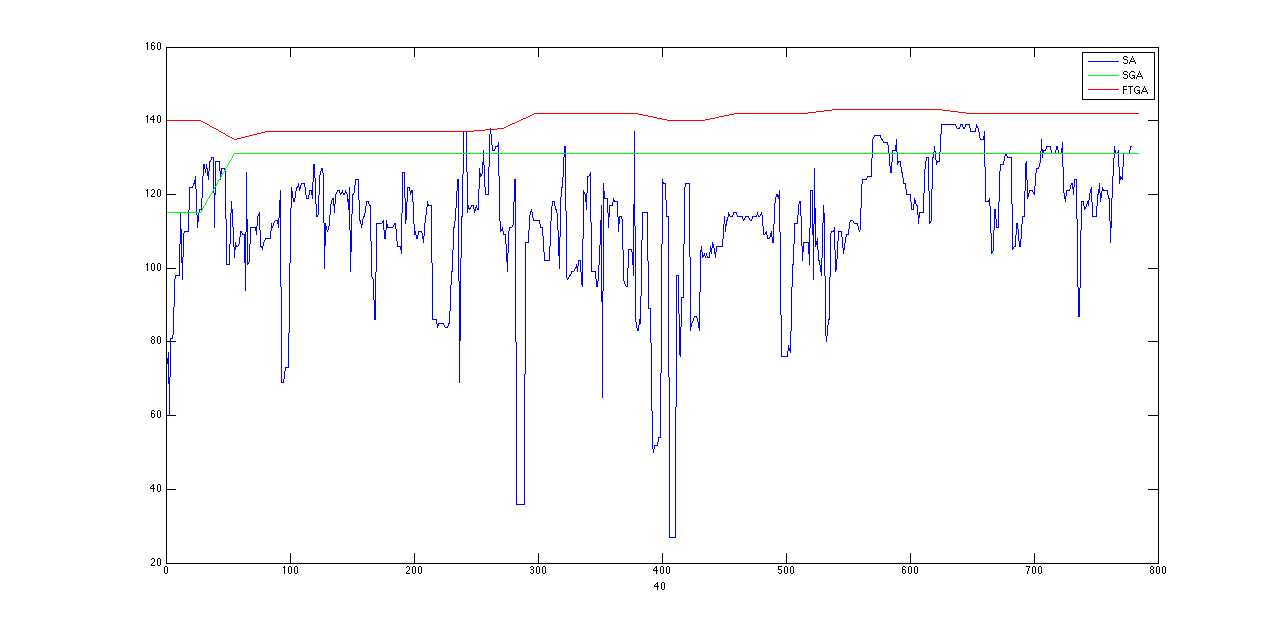
\includegraphics[scale=0.3]{images/FTGA/exp1/30.png}
\caption{Generation = 30}
\end{figure}
\begin{figure}[H]
\centering
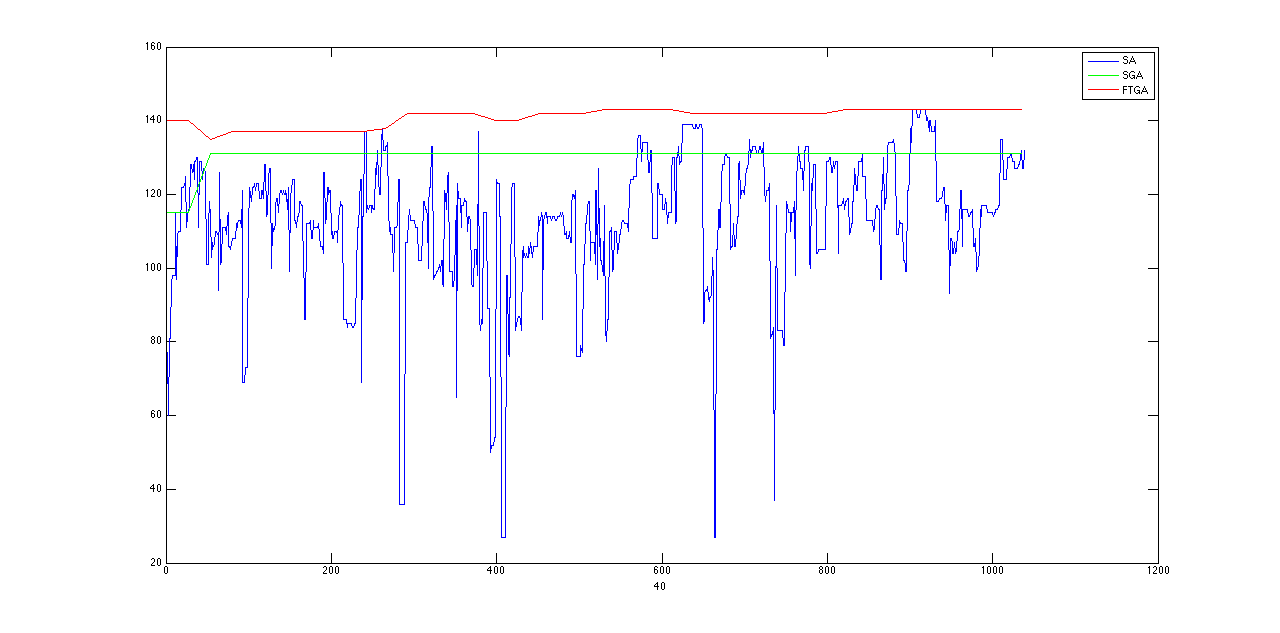
\includegraphics[scale=0.3]{images/FTGA/exp1/40.png}
\caption{Generation = 40}
\end{figure}

\subsection{Experiment Conclusion}
From the previous section, we can see how these algorithms perform. The red line represents the performance of FTGA in each figure. The green line represents the performance of SGA and the blue line represents SA. It is normal for the fitness of SA to fluctuate during the whole process and its fitness finally goes to the maximum value that it can achieve. SGA has a relative high fitness in the very beginning, then it gets stuck at some local optimum. FTGA performs the best among these three algorithms. 

\subsection{Footnotes}

Indicate footnotes with a number\footnote{Sample of the first footnote} in the
text. Place the footnotes at the bottom of the page on which they appear.
Precede the footnote with a horizontal rule of 2~inches
(12~picas).\footnote{Sample of the second footnote}

\subsubsection*{Acknowledgments}

Use unnumbered third level headings for the acknowledgments. All
acknowledgments go at the end of the paper. Do not include 
acknowledgments in the anonymized submission, only in the 
final paper. 

\subsubsection*{References}

References follow the acknowledgments. Use unnumbered third level heading for
the references. Any choice of citation style is acceptable as long as you are
consistent. It is permissible to reduce the font size to `small' (9-point) 
when listing the references. {\bf Remember that this year you can use
a ninth page as long as it contains \emph{only} cited references.}

\small{
[1] Alexander, J.A. \& Mozer, M.C. (1995) Template-based algorithms
for connectionist rule extraction. In G. Tesauro, D. S. Touretzky
and T.K. Leen (eds.), {\it Advances in Neural Information Processing
Systems 7}, pp. 609-616. Cambridge, MA: MIT Press.

[2] Bower, J.M. \& Beeman, D. (1995) {\it The Book of GENESIS: Exploring
Realistic Neural Models with the GEneral NEural SImulation System.}
New York: TELOS/Springer-Verlag.

[3] Hasselmo, M.E., Schnell, E. \& Barkai, E. (1995) Dynamics of learning
and recall at excitatory recurrent synapses and cholinergic modulation
in rat hippocampal region CA3. {\it Journal of Neuroscience}
{\bf 15}(7):5249-5262.
}

\end{document}
